\documentclass[%
 aip,
 jmp,%
 amsmath,amssymb,
%preprint,%  comment out to make pretty
reprint,% uncomment to make pretty
%author-year,%
%author-numerical,%
]{revtex4-1}

\usepackage{tikz}

\usepackage{graphicx}% Include figure files
\usepackage{dcolumn}% Align table columns on decimal point
\usepackage{bm}% bold math
\usepackage{outlines}
\begin{document}

\title{Optimized gustatory perception of french pressed Coffea arabica and Coffea canephora}

\author{Timothy C. Moore}
\author{Andrew Z. Summers}
\author{Christoph Klein}
\affiliation{Department of Chemical and Biomolecular Engineering, Vanderbilt University, Nashville, Tennessee 37235, United States}
\affiliation{Vanderbilt Multiscale Modeling \& Simulation Center, Vanderbilt University, Nashville, Tennessee 37235, United States}

\author{Casey Brock}
\affiliation{Vanderbilt Multiscale Modeling \& Simulation Center, Vanderbilt University, Nashville, Tennessee 37235, United States}
\affiliation{Department of Mechanical Engineering, Vanderbilt University, Nashville, Tennessee 37235, United States}


\date{\today}

\begin{abstract}
Your abstract
\end{abstract}

\maketitle

\section{Introduction}


\section{Methods}
\begin{outline}[enumerate]
\1 Coffee was prepared in a Bodum Brazil 8-Cup French Press Coffee Maker
\end{outline}
\begin{figure}
    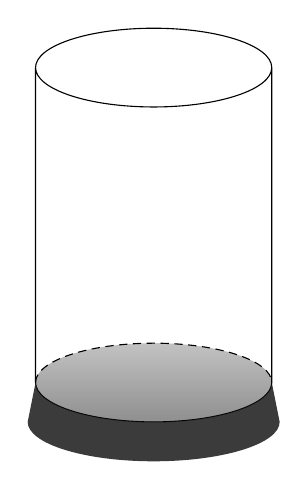
\begin{tikzpicture}
\fill[top color=gray!40, bottom color=black, shading=axis, opacity=0.25] (0,0) circle (1.5cm and 0.5cm); %bottom grayness
\draw (-1.5,4) -- (-1.5,0) arc (180:360:1.5cm and 0.5cm) -- (1.5,4) ++ (-1.5,0) circle (1.5cm and 0.5cm); %bottom front circle
\draw[densely dashed] (-1.5,0) arc (180:0:1.5cm and 0.5cm); %bottom back dashed circle

\fill[color=black!90, opacity=0.85] (-1.6,-0.5) -- (-1.5,0) arc (180:360:1.5cm and 0.5cm) -- (1.6,-0.5) arc (180:360:-1.6cm and 0.5cm); %base front circle

\fill[color=black!90, opacity=0.85] ; %handle
\end{tikzpicture} 
    \caption{Schematic of Bodum french press}
    \label{fig:press_diagram}
\end{figure}

\section{Results}


\section{Conclusions}



\bibliography{french-press-study.bib}

\end{document}





